\documentclass[a4paper]{article}

\usepackage[T1]{fontenc}
\usepackage[utf8]{inputenc}

\usepackage{mathptmx}

\usepackage[a4paper, total={6in, 8in}]{geometry}
\usepackage{subcaption}
\usepackage[shortlabels]{enumitem}
\usepackage{amssymb}
\usepackage{amsthm}
\usepackage{mathtools}
\usepackage{braket}
\usepackage{bbm}
\usepackage{graphicx}
\usepackage{float}
\usepackage{yhmath}
\usepackage{tikz}
\usetikzlibrary{calc,decorations.markings}
\usepackage[colorlinks=true,naturalnames=true,plainpages=false,pdfpagelabels=true]{hyperref}
\usepackage[parfill]{parskip}
\usepackage[backend=biber, sorting=none]{biblatex}
\newcommand{\hbbar}{{\raisebox{0.05ex}{$\mathchar '26$}\mkern -9mu\raisebox{-0.15ex}{$\mathchar '26$}\mkern -9muh}}
\addbibresource{uni.bib}
\pagestyle{myheadings}
\markright{Popovic, Vogel\hfill Dispertion relations \hfill}


\title{Universität Wien\\ Fakultät für Physik\\
\vspace{1.25cm}Laborpraktikum Theoretische Physik 2021S \\ Dispersion relations
}
\author{Milutin Popovic \& Tim Vogel \vspace{1cm}\\ Betreuer: Peter Stoffer}
\date{30. Juni, 2021}

\begin{document}
\maketitle
\noindent\rule[0.5ex]{\linewidth}{1pt}
\begin{abstract}
This protocol will provide a first look at dispersion relations. We will show
some trivial examples in the harmonic oscillator, where the mathematical basics
are provided and applied. From this we will dive into more complex topics,
derive a few equations within scattering processes in quantum dynamics and
after that, show, that dispersion do not only work in the quantum physical
world, but also find application in particle physics, where they can be used to
obtain results in areas, where quantum chromodynamics fail. We explicitly
calculate solutions to the so called Omnés-problem, and finally apply some
numerical values to the found solutions.
\end{abstract}
\noindent\rule[0.5ex]{\linewidth}{1pt}
\newcommand{\PV}{\mathop{\mathrlap{\pushR}}\!\int}
\newcommand{\pushR}{\mathchoice
  {\mkern2.5mu P}
  {\scriptstyle P}
  {\scriptscriptstyle P}
  {\scriptscriptstyle P}
}

\tableofcontents
\section{Introduction}
Within the tools of complex analysis, there exists the possibility, to form
relations between observable quantities of physicals systems, for example
dispersion in a dielectric medium. This can be taken even further, by using the
same methods within particle-physical problems, where the now more popular
methods of quantum chromodynamics do not apply, which would be low energy
hadronic processes. We will firstly apply these concepts to the simple example
of the harmonic oscillator and finally work out more complex problems,
regarding the pion vector form factor. The reader is expected to be familiar
with the subject of complex analysis, especially analyticity/holomorphicity of
a function, integration of complex functions, the residue theorem and the
Schwartz reflection principle.

\section{Damped harmonic oscillator}
Considering a free harmonic oscillator, the equation of motion accounts to:
\begin{equation}
    \Ddot{x}(t)+\gamma\Dot{x}(t)+\omega_0^2x(t)=0
\end{equation}
where $\gamma > 0$ is the damping coefficient, and $\omega_0$ the angular frequency
of the oscillator. Using the exponential ansatz we can arrive at an general
solution to this ordinary differential equation
\begin{align}
    &x(t) = a e^{-i\omega_1 t} + b e^{-i\omega_2 t} \\
    &\nonumber \\
    \text{with:} \nonumber\\
    &\omega_{1/2} = \pm \sqrt{\omega_0^2 - (\frac{\gamma}{2})^2} -
    i\frac{\gamma}{2}
\end{align}
where $a$ and $b$ are calculated based on the Couchy boundary conditions.

For the case $\omega_0 > \frac{\gamma}{2}$ we can rewrite the solution
\begin{align}
    &x(t) = \left(a e^{-i\tilde{\omega}_0 t} + b e^{-i\tilde{\omega}_0
    t}\right) e^{-\frac{\gamma}{2}t}\\
    &\nonumber \\
    \text{with:} \nonumber\\
    &\tilde{\omega}_{0} = \sqrt{\omega_0^2 - \left(\frac{\gamma}{2}\right)^2}
\end{align}
\subsection{External Force}

Now consider a harmonic oscillator with an external force $F(t)$ driving it
\begin{align}\label{eq:force}
    \Ddot{x}(t)+\gamma\Dot{x}(t)+\omega_0^2x(t)=\frac{F(t)}{m} =: f(t).
\end{align}
By Fourier transforming the equation we can arrive at an equation for the
greens function in Fourier space. Note that the Fourier transform of
$x(t)$ is
\begin{align}
   \hat{x}(t) &= \frac{1}{2\pi}\int_\infty^\infty d\omega
    X(\omega) e^{-i\omega t}
\end{align}
so the Fourier transforms of $\dot{x}$ and $\Ddot{x}$ are
\begin{align}
    \mathcal{F}(\dot{x}) &= -i\omega X(\omega)\\
    \mathcal{F}(\Ddot{x}) &= -\omega^2 X(\omega)\\
\end{align}
and the equation \ref{eq:force} turns into
\begin{align}
    (-\omega^2 - i\gamma \omega + \omega_0^2) X(\omega) = F(\omega)
\end{align}

The Green's function can be represented in Fourier space like the following
\begin{align}
    G(\omega)= \frac{1}{-\omega^2 - i\gamma \omega + \omega_0^2}
\end{align}

The Maximum of the squared modulus $|G(\omega)|^2$ for $\gamma \ll \omega_0$ is
roughly at $\omega_0$, thus the width at half maximum can be calculated by
looking for two $\omega$'s that satisfy
\begin{align}
    \frac{1}{2}|G(\omega_0)|^2 &= |G(\omega)|^2\\
    \frac{1}{2} \frac{1}{\omega_0^2\gamma^2} &= |G(\omega)|^2
\end{align}

The exact solutions are
\begin{align}
    \tilde{\omega}_1 &= \omega_0\sqrt{-0.5\left(\frac{\gamma}{\omega_0}\right)^2
    - 1.0\frac{\gamma}{\omega_0}(0.25\left(\frac{\gamma}{\omega_0}\right)^2
    + 1)^{\frac{1}{2}} + 1}\\
    \tilde{\omega}_2 &= \omega_0\sqrt{-0.5\left(\frac{\gamma}{\omega_0}\right)^2
    + 1.0\frac{\gamma}{\omega_0}(0.25\left(\frac{\gamma}{\omega_0}\right)^2
    + 1)^{\frac{1}{2}} + 1}
\end{align}
With help of Taylor expansion in the linear order in $\frac{\gamma}{\omega_0}$
gives us the approximation for the with at half maximum
\begin{align}
    \tilde{\omega}_2 - \tilde{\omega}_1 \simeq \gamma
\end{align}

In the figure below we plotted the squared modulus of $|G(\omega)|^2$
\begin{figure}[H]
    \centering
    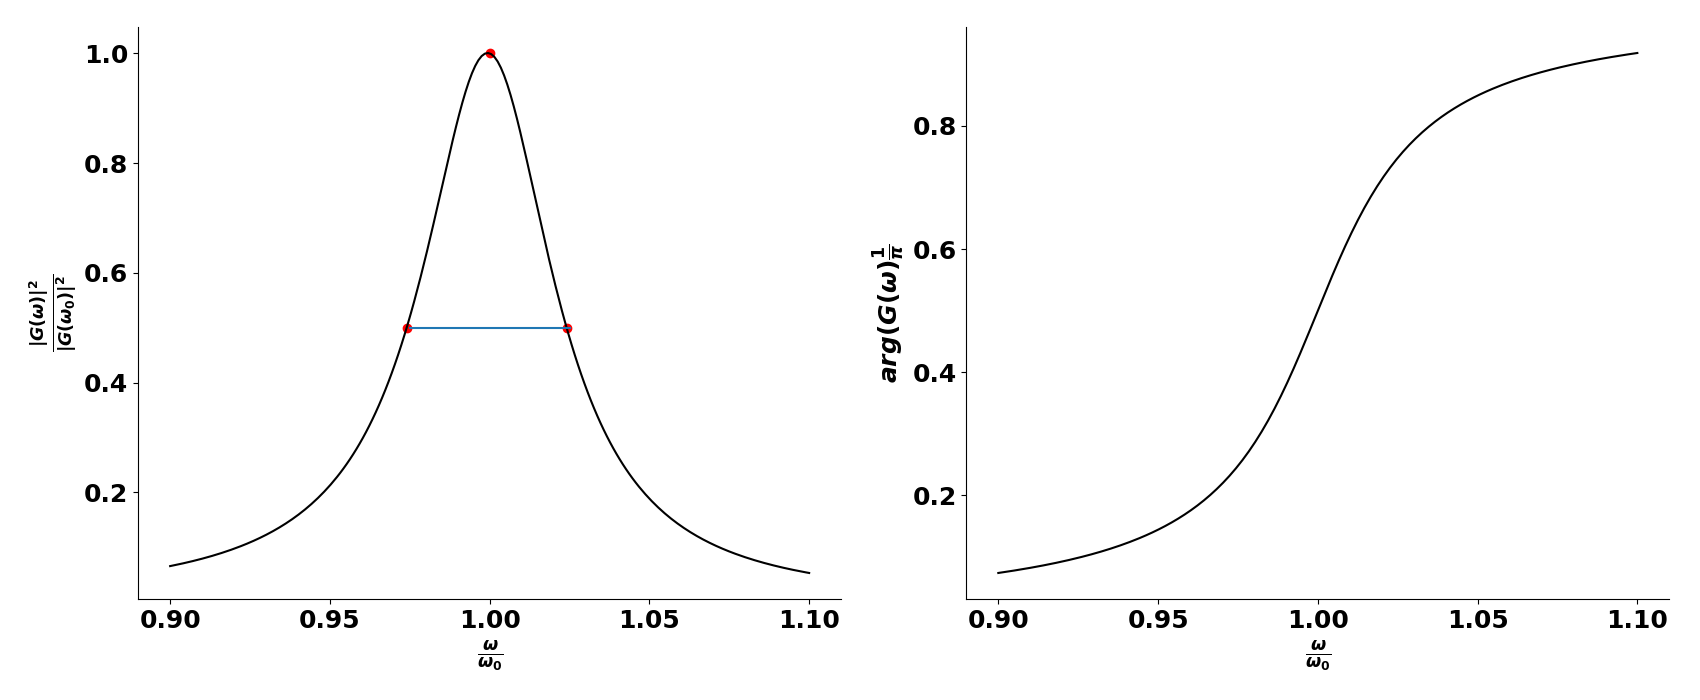
\includegraphics[width=\textwidth]{section2.png}
    \caption{On the left the squared modulus $|G(\omega)|^2$ in $\omega
\in [\omega_0 - 2\gamma, w_0 + w\gamma]$ for $\gamma \ll \omega_0$, precisely
$\gamma = \omega_0/20$ for $\omega_0 = 1$ and on the right $arg(G(\omega))$}
\end{figure}


Next we want calculate the Green's function in terms of time
\begin{align}
    g(t) = \frac{1}{2\pi} \int^\infty_\infty d\omega G(\omega)e^{-i\omega t}.
\end{align}
Furthermore we can transform this to the complex integral where we have two singularities
at We have two singularities at $z_{1/2} =  - \frac{i\gamma}{2} \pm
\tilde{\omega}_{0}$. We have the following integral
path

\begin{center}
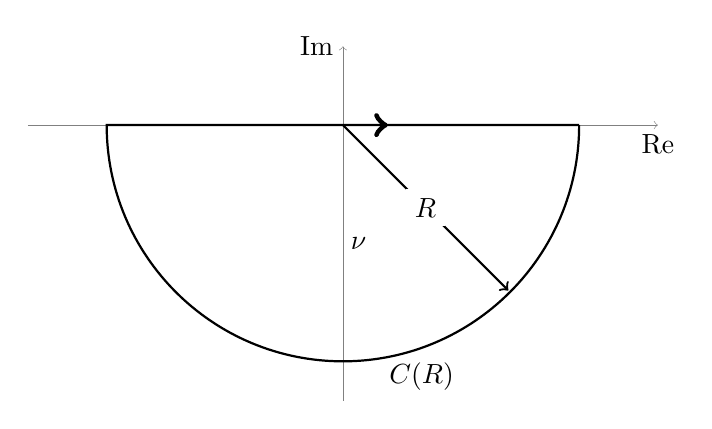
\begin{tikzpicture}[decoration={markings,
mark=at position 13cm with {\arrow[line width=2pt]{>}}
}
]
% The axes
\draw[help lines,->] (-4,0) -- (4,0) coordinate (xaxis);
\draw[help lines,->] (0,-3.5) -- (0,1) coordinate (yaxis);

% The path
\path[draw,line width=0.8pt,postaction=decorate]
    (3,0) node[above right] {} arc (0:-180:3) -- (-3, 0)
    node[above left] {} -- (-3, 0) -- (3, 0);

% The labels
    \draw[thick, ->] (0,0) -- (2.1, -2.1) node[midway, fill=white] {$R$};
    \node[below] at (xaxis) {$\text{Re}$};
    \node[left] at (yaxis) {$\text{Im}$};
    \node at (0.2,-1.5) {$\nu$};
    \node at (1, -3.2) {$C(R)$};
\end{tikzpicture}
\end{center}

The complex integral representation is
\begin{align}
    \oint_\nu dz G(z) e^{-izt} &=
     \lim_{R \rightarrow \infty }
     \bigg(
    \int_{C(R)} + \int_{-R}^{R}
    \bigg)
    dz\ G(z) e^{-izt}\\
    &= 2\pi i\sum_j \text{I}(C_j, z_j) \text{Res}_j
\end{align}
Keep in mind that the integral from $R$ to $-R$ is the integral we are
trying to solve, that is pulling the limit we have one integral over the real
axis. Because of Jordan's lemma, the integral over the complex curve vanishes
\begin{align}
    \big| \int_{C(R)} dz G(z) e^{-izt}\big| \leq \frac{\pi}{t}M_R
\end{align}
where $M_R:= \max_{C(R)}\{G(Re^{i\varphi})\}$.It can easily be seen that $M_R$
converges to $0$ as $R$ goes to infinity. Thus the only value the integral can
take is $0$ and we can calculate the real integral with the residues
\begin{align}
    \text{Res}_1 &= \frac{e^{i z t}}{(z - z_1)(z - z_2)} (z - z_1)\bigg|_{z=z_1}
    \\
    &= -\frac{e^{-iz_1t}}{z_1 - z_2} = \frac{e^{-\frac{\gamma}{2}t}
    e^{i\tilde{\omega}_0 t}}{2\tilde{\omega}_0}\\
    \nonumber \\
    \text{Res}_2 &= \frac{e^{i z t}}{(z - z_1)(z - z_2)} (z - z_2)\bigg|_{z=z_2}
    \\
    &= -\frac{e^{-iz_1t}}{z_2 - z_1} = -\frac{e^{-\frac{\gamma}{2}t}
    e^{-i\tilde{\omega}_0 t}}{2\tilde{\omega}_0}\\
\end{align}
with the index $\text{I}(C_R, z_i)$ being $1$, because the curve goes around the
singularities once.

The integral evolves to
\begin{align}
    \frac{1}{2\pi} \int_{-\infty}^{\infty} d\omega G(\omega) e^{-i\omega t}=
    \frac{\sin(\tilde{\omega}_0t)}{\tilde{\omega}_0} e^{-\frac{\gamma}{2}t}.
\end{align}
Treating the cases $t<0$ and $t>0$ separately we can join them with the
Heaviside-theta function $\theta(t)$, the Green's function for the damped
harmonic oscillator is
\begin{align}
    g(t) = \frac{\sin(\tilde{\omega}_0t)}{\tilde{\omega}_0}
    e^{-\frac{\gamma}{2}t} \theta(t)
\end{align}
With convolution we can arrive at a solution for the damped harmonic oscillator
for an arbitrary driving force $f(t)$
\begin{align}
    x(t) = \int_{-\infty}^{t} dt'
    \frac{\sin(\tilde{\omega}_0 (t-t'))}{\tilde{\omega}_0}
    e^{-\frac{\gamma}{2}(t-t')} f(t').
\end{align}

\subsection{Green's Function and dispersion relations}
Next we want to compute the following integral
\begin{align}
    0 = \oint_C d\omega' \frac{G(\omega')}{\omega - \omega'}, \;\;\;\;
    \text{with} \;\;\; \omega' = \omega_r + i\omega_i
\end{align}
along the following contour

\begin{center}
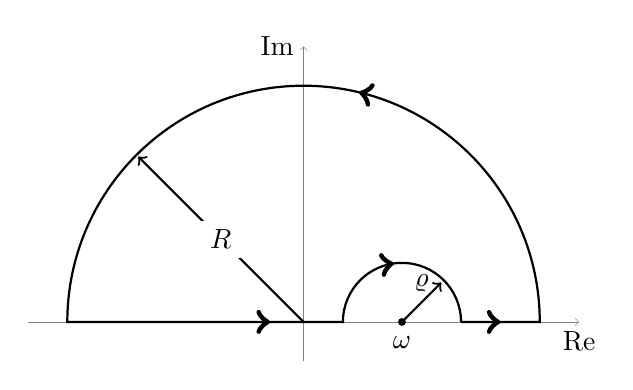
\begin{tikzpicture}[decoration={markings,
mark=at position 0.5cm with {\arrow[line width=2pt]{>}},
mark=at position 5cm with {\arrow[line width=2pt]{>}},
mark=at position 13cm with {\arrow[line width=2pt]{>}},
mark=at position 15cm with {\arrow[line width=2pt]{>}}
}
]
% The axes
\draw[help lines,->] (-3.5,0) -- (3.5,0) coordinate (xaxis);
\draw[help lines,->] (0,-0.5) -- (0,3.5) coordinate (yaxis);

% The path
\path[draw,line width=0.8pt,postaction=decorate]
    (2,0) -- (3, 0) node[below right] {} arc (0:180:3) -- (0.5, 0)
    arc (180:0:0.75);

% The labels
    \draw[thick, ->] (0,0) -- (-2.1, 2.1) node[midway, fill=white] {$R$};
    \draw[thick, ->] (1.25,0) -- (1.75, 0.5) node[midway, above] {$\varrho$};
    \node[below] at (xaxis) {$\text{Re}$};
    \node[left] at (yaxis) {$\text{Im}$};
    \node[circle,inner sep=1pt,label=below:{$\omega$}, fill=black] at (1.25,0) {};
\end{tikzpicture}
\end{center}
so the integral representation is
\begin{align}
    \oint_C d\omega' \frac{G(\omega')}{\omega - \omega'} =
    \lim_{\substack{R\rightarrow \infty \\ \varrho \rightarrow 0^+}}
    \bigg( \int_{C(R)} + \int_{(C(\rho)} + \int_{-R}^{\omega -
    \varrho} + \int_{\omega +\varrho}^R
    \bigg)
    \;d\omega'\ \frac{G(\omega')}{\omega - \omega'}
\end{align}
We need show that the integral over the big circle goes to $0$. We know that for
$\omega' \neq \omega$ we have
\begin{align}
    \big|\frac{G(\omega')}{\omega' - \omega}\big| &=
    \big|\frac{1}{\omega'^3}\frac{1}{(1-\frac{\omega_1}{\omega'})(1-\frac{\omega_2}{\omega'})
    (1 - \frac{\omega}{\omega'})}\big|
    \leq \frac{1}{R^3}
\end{align}
thus
\begin{align}
        \bigg|
    \int_{C(R)} d\omega' \frac{G(\omega')}{\omega - \omega'}
        \bigg| \leq \frac{2\pi R}{R^3} = \frac{2\pi}{R^2}
        \xrightarrow[R\rightarrow \infty]{} 0.
\end{align}
The small circle can be calculated with the Residue theorem with the pole at
$\omega$
\begin{align}
\int_{C(\varrho)}d\omega' \frac{G(\omega')}{\omega - \omega'} = 2\pi i
    \text{I}(C(\varrho), \omega) \text{Res}(\frac{G(\omega')}{\omega - \omega'},
    \omega) = i\pi G(\omega).
\end{align}
Note that we go around $\omega$ only $1/2$ times. Reconstructing the integral
equation we get
\begin{align}
    -i\pi G(\omega) = \lim_{\varrho \rightarrow 0^+}
    \big(
     \int_{-R}^{\omega -\varrho} + \int_{\omega +\varrho}^R
    \big) \;d\omega'\ \frac{G(\omega')}{\omega' - \omega}
\end{align}
which is exactly the Cauchy Principal Value. Furthermore we can rewrite
$G(\omega)$ into real and imaginary parts
\begin{align}
    \text{Re} (G(\omega)) = \frac{1}{\pi} \PV  d\omega' \frac{\text{Im}
    (G(\omega'))}{\omega' - \omega}\\
    \text{Im} (G(\omega)) = \frac{1}{\pi} \PV  d\omega' \frac{\text{Re}
    (G(\omega'))}{\omega' - \omega}\\
\end{align}
which are Hilbert transforms of each other, the equations are also known
as ``dispersion relations''. It should be noted that these equations also allow
negative frequencies. Let us derive an representation for only positive
frequencies. We start off by a simple statement
\begin{align}
    G(-\omega^*) = G(\omega)^*.
\end{align}
In our case this is obviously true
\begin{align}
    &G(-\omega^*) = \frac{1}{-(\omega^*)^2 + i\gamma \omega^* + \omega_0^2}\\
    \nonumber \\
    &G(\omega)^* = \frac{1}{-(\omega^2)^* + i\gamma \omega^* + \omega_0^2} =
    G(-\omega^*)
\end{align}
Now we choose $\omega \in \mathbb{R}^+$, our relation then becomes
$G(-\omega) = G(\omega)^*$. Then we get
\begin{align}
    \text{Re} (G(\omega)) &= \frac{1}{\pi} \PV_0^\infty  d\omega' \frac{2\omega'\text{Im}
    (G(\omega'))}{\omega'^2 - \omega^2}\\
    \text{Im} (G(\omega)) &= -\frac{1}{\pi} \PV_0^\infty  d\omega' \frac{2\omega'\text{Re}
    (G(\omega'))}{\omega'^2 - \omega^2}
\end{align}

To round this chapter up we would like to show one last identity in the sense
of distributions
\begin{align}
    \lim_{\varepsilon \rightarrow 0^+} \frac{1}{\omega' -\omega \mp
    i\varepsilon} = \text{P}(\frac{1}{\omega' - \omega}) \pm i\pi\delta(\omega'
    - \omega).
\end{align}
Let us extend the fraction with $\omega' - \omega \pm i\varepsilon$.
\begin{align}
\frac{\omega' - \omega \pm i\varepsilon}{(\omega' -\omega \mp
    i\varepsilon)(\omega' - \omega \pm i\varepsilon)} = \frac{\omega' - \omega
    \pm i\varepsilon}{(\omega' - \omega)^2 + \varepsilon^2}.
\end{align}
That means for a test function $f(\omega')$ we have
\begin{align}
    \lim_{\varepsilon \rightarrow 0^+} \int_{-\infty}^\infty d\omega'
    \frac{f(\omega')}{\omega' - \omega \mp i\varepsilon} &=
    \lim_{\varepsilon \rightarrow 0^+}
    \int_{-\infty}^\infty d\omega'
    \frac{(\omega' - \omega \pm i\varepsilon) f(\omega')}{(\omega' - \omega)^2
    + \varepsilon^2}\\
    & =
    \lim_{\varepsilon \rightarrow 0^+}\bigg(
    \int_{-\infty}^\infty d\omega'
    \frac{f(\omega')(\omega' - \omega )}{(\omega' - \omega)^2 + \varepsilon^2}
    \pm i\varepsilon
    \int_{-\infty}^\infty d\omega'\frac{f(\omega')}{(\omega' - \omega)^2 + \varepsilon^2}
    \bigg)\label{eq:id}.
\end{align}
Let us look into the first integral in equation \ref{eq:id}, we can rewrite it
\begin{align}
    \lim_{\varepsilon \rightarrow 0^+}\int_{-\infty}^\infty
    d\omega'\frac{f(\omega')(\omega' - \omega )}{(\omega' - \omega)^2 + \varepsilon^2}
    &= \lim_{\varepsilon,\varrho \rightarrow 0^+}
    \bigg(
        \int_{-\infty}^{\omega - \varrho}d\omega'\frac{f(\omega')(\omega' -
        \omega )}{(\omega' - \omega)^2 + \varepsilon^2}
        + \int_{\omega
        \varrho}^{\infty}d\omega'\frac{f(\omega')(\omega' - \omega )}{(\omega'
        - \omega)^2 + \varepsilon^2} + \\
        &+\int_{\omega -\varrho}^{\omega+
        \varrho}d\omega'\frac{f(\omega')(\omega' - \omega )}{(\omega' -
        \omega)^2 + \varepsilon^2}
        \bigg)
        \\
        &= \PV_{-\infty}^{\infty}d\omega' \frac{f(\omega')}{(\omega' - \omega)}
\end{align}
The integral from $\omega - \varrho$ to $\omega + \varrho$ can be calculated by
pulling out $f(\omega)$ out of the integral and directly computing it, which
gives then vanishes. In second integral we approximate $f(\omega')$ to
$f(\omega)$ in the region $\omega' \simeq \omega$
\begin{align}
    \varepsilon \int_{-\infty}^{\infty}d\omega' \frac{f(\omega')}{(\omega' -
    \omega)^2 + \varepsilon^2} &\simeq  \varepsilon f(\omega) \int_{-\infty}^{\infty}
    \frac{1}{(\omega' -\omega)^2 + \varepsilon^2}\\
    &= \pi f(\omega).
\end{align}
Which means the identity is
\begin{align}
    \lim_{\varepsilon \rightarrow 0^+} \int_{-\infty}^{\infty} d\omega'
    \frac{f(\omega')}{\omega' -\omega \mp i\varepsilon} =
    \PV_{-\infty}^{\infty} d\omega' \frac{f(\omega')}{\omega' -\omega} \pm
    i\pi f(\omega)\label{eq:pv}
\end{align}
\section{Potential scattering in quantum mechanics}
If we consider elastic scattering of a spineless particle off a
time-independent, spherically symmetric potential of finite range, we look for
stationary solutions $\psi$ of the Schrödinger equation
\begin{equation}
    -\frac{\hbbar^2}{2m}\Vec{\nabla^2}\psi(\Vec{x})+V(r)\psi(\Vec{x})=E\psi(\Vec{x})
\end{equation}
Since the potential is spherically symmetric, it only depends on $r$ and for
large values of $r$, it can be shown, that the asymptotic form of $\psi$ looks
like:
\begin{equation}
    \psi(r,\theta)\approx A[e^{ikz}+f(E,\theta)\frac{e^{ikr}}{r}]
\end{equation}
Where $kr\gg 1$, and k given by
\begin{equation}
    k=\frac{\sqrt{2mE}}{\hbbar}
\end{equation}
We also define the scattering angle $\theta$ by $z=r\cos{\theta}$, and since
there is no dependence on the azimuthal angle $\phi$. we can define the
incoming and outgoing parts of the wave function as follows:
\begin{equation}
    \psi_{in}=Ae^{ikz}
\end{equation}
and
\begin{equation}
    \psi_{out}=Af(E,\theta)\frac{e^{ikr}}{r}
\end{equation}
Where the factor $\frac{1}{r}$ is carried, to conserve probability. The complex
function $f(E,\theta)$ is the so called scattering amplitude. We are now
interested in the differential cross section $\frac{d\sigma}{d\Omega}$, which
is defined as the ratio of number of particles per unit time, that are
scattered into the surface element $dS=r^2d\Omega(\theta,\phi)$ and the number
of incoming particles per unit time, per are orthogonal to the beam direction.
Expressed via probability currents, we thus obtain:
\begin{equation}
    \frac{d\sigma}{d\Omega}=\frac{\Vec{j}_{out}\cdot \Vec{e}_rr^2}{|\Vec{j}_{in}|}
\end{equation}
With $\Vec{e}_r$ being a unit vector in direction of the radius, and the currents given as:
\begin{equation}
\Vec{j}=\frac{i\hbbar}{2m}(\psi\Vec{\nabla}\psi^*-\psi^*\Vec{\nabla}\psi)
\end{equation}
By applying these equations, we obtain the differential cross section as:
\begin{equation}
    \frac{d\sigma}{d\Omega}=|f(E,\theta)|^2
\end{equation}
With the scattering amplitude, being given as:
\begin{equation}
    f(E,\theta)=\sum_{l=0}^\infty(2l+1)f_l(E)P_l(cos\theta)
\end{equation}
where $l$ denotes the magnitude of orbital angular momentum, and
$P_l(cos\theta)$ are the Legendre polynomials.
We can now work out the total cross section $\sigma$ via the integral:
\begin{equation}
    \sigma=\int{d\Omega\frac{d\sigma}{d\Omega}}
\end{equation}
We do this, by applying the orthogonality relation
\begin{equation}
    \int{d\Omega P_l(cos\theta)P_{l'}(cos\theta)}=\frac{4\pi}{(2l+1)}\delta_{ll'}
\end{equation}
Thus, we obtain:
\begin{equation}
    \sigma=\sum_{l,l'}(2l+1)(2l'+1)f^*_l(E)f_{l'}(E)\int{d\Omega
    P_l(cos\theta)P_{l'}(cos\theta)}
\end{equation}
Which, finally leads to:
\begin{equation}
    \sigma=4\pi\sum_l(2l+1)|f(E)|^2
\end{equation}
By now defining a phase shift of:
\begin{equation}
    S_l(k)=1+2ikf_l(E)
\end{equation}
where, $S_l(k)$ is the $l$-th matrix element of the scattering operator, and
can also be written as:
\begin{equation}
    S_l=e^{2i\delta_l}
\end{equation}
Thus, one can see pretty quickly, that
\begin{equation}
    f_l(E)=\frac{e^{2i\delta_t}-1}{2ik}=\frac{e^{i\delta_l}\sin{\delta_l}}{k}
\end{equation}
With this result, we can now derive the optical theorem. We start, by plugging
the result above into equation (66)
\begin{equation}
    \sigma=4\pi\sum_{l=0}^\infty
    (2l+1)|\frac{1}{k}e^{i\delta_lE}\sin{\delta_l(E)}|^2
    =\frac{4\pi}{k^2}\sum_l (2l+1)\sin^2{\delta_l}
\end{equation}
with
\begin{equation}
    Im\, f(E,0)=\sum_{l=0}^\infty
    (2l+1)Im(\frac{e^{i\delta_l}}{k})\sin{\delta_l}=\frac{1}{k}\sum_l
    (2l+1)\sin^2{\delta_l}
\end{equation}
Which, finally leads to:
\begin{equation}
    \sigma_{el}=\frac{4\pi}{k}Im\, f(E,0)
\end{equation}
We now consider a froward scattering amplitude, with the asymptotic behavior
$[f(E,0)-f_\infty(0)]\rightarrow E^{}-1-\epsilon$ for $|E|\rightarrow\infty$,
with $\epsilon>0$. We want to compute the integral, given by:
\begin{equation}
    \oint_\Gamma dE'\frac{f(E',0)-f_\infty(0)}{E'-E}=2\pi i\sum_i^N\frac{Res_{E'=E_i(f(E',0)-f_\infty(0)}}{E_i-E}
\end{equation}
From the optical theorem we know, that the forward scattering amplitude is real
on the negative real axis, and we also assume that $F_\infty(0)$ is real, as
well. For further calculations the integrand in equation (73) will be named
$F(E')$, to improve readability, also the arguments of the functions $f(E,0)$
and $f_\infty(0)$ will be left out, from this point forward. Firstly, we
consider the parts of the curve, parallel to the real axis. We say $f(E,0)$ is
analytical on the upper half plane, to the point E. By making use of the
Schwarz reflection principle, we can write:
\begin{equation}
    \int_\leftarrow dE'F(E'^*)+\int_\rightarrow dE'F(E')=\int_\leftarrow
    dE'F^*(E')+\int_\rightarrow dE'F(E')=2i\int\rightarrow dE'\, ImF(E')
\end{equation}
The imaginary part of $F(E')$ equates to:
\begin{equation}
    Im(F)=Im(\frac{f-f_\infty}{E'-E})=\frac{1}{|E'-E|^2}[Im(f)Re(E'-E)-Re(f)Im(E'-E)+f_\infty
    Im(E'-E)]
\end{equation}
We can now calculate the residues of each term of equation (75) individually.
To achieve this, we consider the point $E=E_r+\alpha iE_i$. We will start by
calculating the residues for the second and third term first, since the first
term will be used differently. So, for the second term, we obtain the residue
as follows:
\begin{equation}
    Res_{E_2}=\lim\limits_{\alpha\rightarrow
    0}\frac{d}{dE'}(E'-E)^2\frac{Re(f)Im(E'-E)}{(E'-E)(E'-E)^*}|_{E'=E}
\end{equation}
\begin{equation}
    =\lim\limits_{\alpha\rightarrow
    0}\frac{d}{dE'}\frac{Re(f)Im(E'-E)(E'-E)}{(E'-E)^*}|_{E'=E}
\end{equation}
The product rule leaves four terms to calculate from this equation, but three
of which can be disregarded, since they vanish, if the limit is taken before
the derivation. The last term comes to:
\begin{equation}
    \frac{d}{dE'}Im(E'-E)=-\frac{i}{2}
\end{equation}
Which leaves the residue as:
\begin{equation}
   Res_{E_2}=-\frac{i}{2}Ref(E)
\end{equation}
By the same procedure, the other residue amounts to:
\begin{equation}
    Res_{E_3}=-\frac{i}{2}f_\infty
\end{equation}
For the first term, we calculate the integral
\begin{equation}
   \lim\limits_{\alpha\rightarrow 0}\int_0^\infty dE'\frac{Imf(E',0)}{|E'-E|^2}=P\int_0^\infty dE'\frac{Imf(E',0)}{E'-E}+\int_{circle}dE'\frac{Imf(E',0)}{|E'-E|^2}
\end{equation}
Where $P\int$ denotes the principal value integral. With $E'=E_r-\rho e^{i\phi}$ and $E=E_r+i\alpha E_i$, the seconds integral in equation (81) can be written as
\begin{equation}
    \lim\limits_{\alpha\rightarrow 0}\lim\limits_{\rho\rightarrow 0}\int_\pi^{2\pi}d\phi\frac{Imf(E_r-\rho e^{i\phi},0)(\rho\cos{\phi})}{|(E_r-\rho e^{i\phi})-(E_r+i\alpha E_i)|^2}(-i\rho e^{i\phi})\rightarrow 0
\end{equation}
Thus, we finally obtain:
\begin{equation}
    \oint_\Gamma dE'\frac{f(E',0)-f_\infty(0)}{E'-E}=2i(-\pi Ref(E',0)+\pi f_\infty(0)+P\int_0^\infty dE'\frac{Imf(E',0)}{E'-E})
\end{equation}
Which is equal to
\begin{equation}
    Ref(E',0)=f_\infty(0)+\frac{1}{\pi}P\int_0^\infty dE'\frac{Imf(E',0)}{E'-E}-\sum_i^N\frac{Res_{E'=E_i}(f(E',0)-f_\infty(0))}{E_i-E}
\end{equation}

\section{The pion vector from factor and the Omn\`es Problem}
Not only do the principles of unitarity and analyticity apply in quantum
physical scattering processes, they also work very well within relativistic
ones in quantum field theory. For processes involving the strong nuclear force,
quantum chromodynamics describe the involved theory. While for high energies,
the very usual way, of perturbative expansion works very well, the smaller the
energy the more unreliable the perturbative schemes get. The advantage of
dispersion relations is now, that they hold non-perturbatively and thus
enabling us, to obtain results by plugging in experimental input and deriving
relations between observables. One such application is the pion vector form
factor, which describes the non-perturbative effects of the strong interaction,
affecting the transition of the virtual photon into the pion pair, in a
collision between an electron and its anti-particle. The so called Omnés
problem describes a way to find the pion VFF, via the $\pi\pi$ - phase shift.
\subsection{Unitarity of the scattering matrix}
As in quantum mechanics, we also define a scattering matrix in particle
physics. This S-matrix describes the transition of incoming particles into
outgoing particles in a scattering experiment. The S-operator must be unitary,
in order to preserve probability and not to change the norm of the state:
\begin{equation}
    SS^\dagger=S^\dagger S=1
\end{equation}
This can be used to obtain Watson's final state theorem:
\begin{align}
    \label{eq:rec}
    \text{Im}(F^V_\pi(s) = F^V_\pi(s) e^{-i\delta_{\pi\pi}(s)}\sin\delta_{\pi\pi}(s)
\end{align}
\subsection{The Omn\`es Problem}
The equations \ref{eq:rec} allow us to carefully reconstruct the pion Vector Form
Factor, based on strictly formulated conditions. This is known as the Omn\`es
Problem. First of all the equation tells us that $F_\pi^V(s)$ is a complex
valued function, as $s$ is an analytic variable in the complex plane, apart
from a cut complex s-plane $\Gamma = [s_0, \infty) \subset \mathbb{R}$, where
$s_0 = 4M_\pi^2 > 0$. To summarize e the conditions are
\begin{itemize}
    \item $F_\pi^V(s)$ is analytic on the cut complex s-plane
        $\mathbb{C}\backslash \Gamma$
    \item $F_\pi^V(s)\in \mathbb{R} \;\;\; \forall\; s \in
        \mathbb{R}\backslash \Gamma$
    \item $\lim_{\varepsilon \rightarrow 0}(F_\pi^V(s+i\varepsilon)
        e^{-i\delta_{\pi\pi}(s)}) \in \mathbb{R}$ on $\Gamma$ for a real
        bounded function $\delta_{\pi\pi}(s)$
    \item We assume $F_\pi^V(0) = 1$ and $F_\pi^V(s)$ has no zeros.
\end{itemize}
We start off with the Couchy Integral
\begin{align}
    \ln(F(s)) = \frac{1}{2\pi i}\oint_C ds' \frac{\ln(F(s'))}{s'-s}
\end{align}
over the following contour
\begin{center}
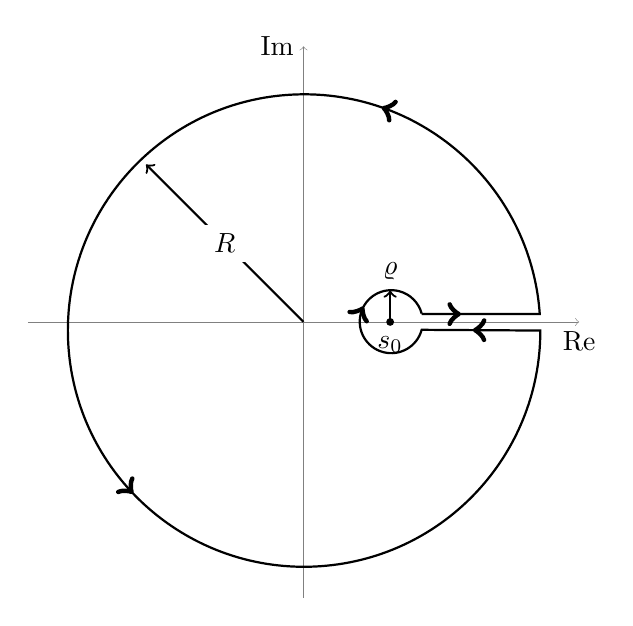
\begin{tikzpicture}[decoration={markings,
mark=at position 0.5cm with {\arrow[line width=2pt]{>}},
mark=at position 5cm with {\arrow[line width=2pt]{>}},
mark=at position 13cm with {\arrow[line width=2pt]{>}},
mark=at position 21cm with {\arrow[line width=2pt]{>}},
mark=at position 23cm with {\arrow[line width=2pt]{>}}
}
]
% The axes
\draw[help lines,->] (-3.5,0) -- (3.5,0) coordinate (xaxis);
\draw[help lines,->] (0,-3.5) -- (0,3.5) coordinate (yaxis);

% The path
\path[draw,line width=0.8pt,postaction=decorate]
    (1.5,0.1) -- (3, 0.1) node[below right] {} arc (4:360:3) -- (1.5, -0.1)
    node[below right] {} arc(345:15:0.4);

% The labels
    \draw[thick, ->] (0,0) -- (-2, 2) node[midway, fill=white] {$R$};
   \draw[thick, ->] (1.1,0) -- (1.1, 0.4) node[above] {$\varrho$};
    \node[below] at (xaxis) {$\text{Re}$};
    \node[left] at (yaxis) {$\text{Im}$};
    \node[circle,inner sep=1pt,label=below:{$s_0$}, fill=black] at (1.1,0) {};
\end{tikzpicture}
\end{center}
This means the integral can be separated into
\begin{align}
    \oint_C ds' \frac{\ln(F(s'))}{s'-s} =
    \lim_{\substack{\varepsilon \rightarrow 0}}
    \bigg(
    \int_{C(R)} + \int_{C(\varrho)} + \int_{s_0+i\varepsilon}^{\infty
    +i\varepsilon} +  \int^{s_0-i\varepsilon}_{\infty
    -i\varepsilon}
    \bigg) ds' \frac{\ln(F(s'))}{s'-s}
\end{align}
The integrals over $C(R)$ and $C(\varrho)$ disappear. For the last two
integrals we can use the Schwarz reflection principle and then we get
\begin{align}
    \oint_C ds' \frac{\ln(F(s'))}{s'-s} = \frac{1}{\pi} \int_{s_0}^{\infty}ds'
    \text{Im}\left(
    \frac{\ln(F(s'))}{s'-s}\right)
\end{align}
where we used $\text{Im}(z) = \frac{z - z^*}{2i}$ to write the imaginary part
here. We look now at equation \ref{eq:rec} and refactor it
\begin{align}
    &\frac{F_\pi^V(s)-F_\pi^V(s)^*}{2i} = F_\pi^V e^{i\delta_{\pi\pi}}(s)
    \sin(\delta_{\pi\pi}(s)) \\
    &F_\pi^V(s) = F_\pi^V(s)^* e^{2i \delta_{\pi\pi}(s)}\\
    &\ln(F_\pi^V(s)) = \ln((F_\pi^V e^{-i\delta_{\pi\pi}})^*)+
    i\delta_{\pi\pi}(s).\label{eq:use}
\end{align}
Now we use this equation to compute the integral with variation in $s
\rightarrow s+i\varepsilon$ as $\varepsilon$ goes to infinity.
\begin{align}
    \ln(F_\pi^V(s)) &= \lim_{\substack{\varepsilon \rightarrow \infty}}
    \ln(F_\pi^V(s+i\varepsilon)) = \\
    &= \lim_{\substack{\varepsilon \rightarrow \infty}}\frac{1}{\pi}
    \int_{s_0}^{\infty}
    \text{Im}\left(\frac{F_\pi^V(s')}{s'-s-i\varepsilon}\right)=\\
    &=\lim_{\substack{\varepsilon \rightarrow \infty}}\frac{1}{\pi}
    \int_{s_0}^{\infty}
    \text{Im}\left(\frac{\ln((F_\pi^V e^{-i\delta_{\pi\pi}})^*)+
    i\delta_{\pi\pi}}{s'-s-i\varepsilon}\right)
\end{align}
the part $F_\pi^V e^{-i\delta_{\pi\pi}}$ needs to be real that means
\begin{align}
    \ln(F_\pi^V(s)) &= \lim_{\substack{\varepsilon \rightarrow \infty}}\frac{1}{\pi}
    \int_{s_0}^{\infty}
    \frac{\delta_{\pi\pi}(s')}{s'-s-i\varepsilon} =\\
    &= \ln(F_\pi^V(0)) + \lim_{\substack{\varepsilon \rightarrow \infty}}
    \frac{s}{\pi}
    \int_{s_0}^{\infty}
    \frac{\delta_{\pi\pi}(s')}{s'(s'-s-i\varepsilon)}
\end{align}
with the condition $F_\pi^V(0) = 1$ and the relation from \ref{eq:pv} we get
\begin{align}
    F_\pi^V(s) =  \exp
    \bigg(
        \frac{s}{\pi}\PV_{s_0}^\infty ds' \frac{\delta_{\pi\pi}(s')}{s'(s'-s)}
        + i\delta_{\pi\pi}(s)
    \bigg).
\end{align}
To compute the principal value integral we use the following trick
\begin{align}
    \frac{s}{\pi}\PV_{s_0}^\infty ds' \frac{\delta_{\pi\pi}(s')}{s'(s'-s)} =
    \frac{s}{\pi} \int_{s_0}^\infty ds' \frac{\delta_{\pi\pi}(s')
    -\delta_{\pi\pi}(s)}{s'(s'-s)}+
    \delta_{\pi\pi}\frac{s}{\pi}\PV_{s_0}^\infty \frac{1}{s'(s'-s)}.
\end{align}
The first integral can be computed numerically, the second one has an analytic
solution for $s > s_0$. We use the definition of the principal value and circle
around $s$ in a small half circle with the radius $r$.
\begin{align}
    \PV_{s_0}^\infty \frac{1}{s'(s'-s)} = \lim_{\substack{r\rightarrow0}}
    \bigg(
    \int_{s_0}^{s-r}ds'  + \int_{s+r}^{\infty} ds'
    \bigg)\frac{1}{s'(s'-s)}
\end{align}
then we simply integrate and plug in
\begin{align}
    \PV_{s_0}^\infty \frac{1}{s'(s'-s)} &= \lim_{\substack{r\rightarrow 0}}
    \bigg(
    \frac{\ln(s'-s) - \ln(s')}{s}\big|_{s'= s_0}^{s'= s-r}
    \frac{\ln(s'-s)-\ln(s')}{s}\big|_{s'=s+r}^{s'=\infty}
    \bigg) =\\
    &=\frac{1}{s}\ln\left(\frac{s_0}{s_0-s}\right)
\end{align}
that means the second integral is
\begin{align}
    \delta_{\pi\pi}\frac{s}{\pi}\PV_{s_0}^\infty \frac{1}{s'(s'-s)}
    =\delta_{\pi\pi}(s)\frac{1}{\pi} \ln\left(\frac{s_0}{s_0 -s }\right)
\end{align}

Lastly we would like to plot the modulus of the Omn\`es representation of the
pion vector form
factor. For the phase we would usually use experimental values, but in our case
we will use the Breit-Wigner representation of the pion VVF to compute the
phase $\delta_{\pi\pi}$. A reminder the Breit-Wigner representation is the
following
\begin{align}
    F^V_\pi(s)_{BW} = \frac{M_\varrho^2}{M_\varrho^2 - s - iM_\varrho
    \Gamma_\varrho(s)}
\end{align}
where
\begin{align}
    \Gamma_\varrho(s) := \Gamma_\varrho\frac{s}{M_\varrho^2} \left(
    \frac{\sigma_\pi(s)}{\sigma_\pi(M_\varrho^2)}
    \right)^3 \theta(s-4M_\pi^2), \;\;\;\;\;\; \sigma_\pi(s) :=
    \sqrt{1-\frac{4M_\pi^2}{s}}.
\end{align}
Thus our phase shift will be
\begin{align}
    \delta_{\pi\pi}(s) := \arg\left(F_\pi^V(s)_{BW}\right)
\end{align}
where we will use numerical values for $M_\varrho = 0.77\ \text{GeV}$,
$\Gamma_\varrho = 0.15\ \text{GeV}$, $M_\pi = 0.14 \text{GeV}$.
\begin{figure}[H]
    \centering
    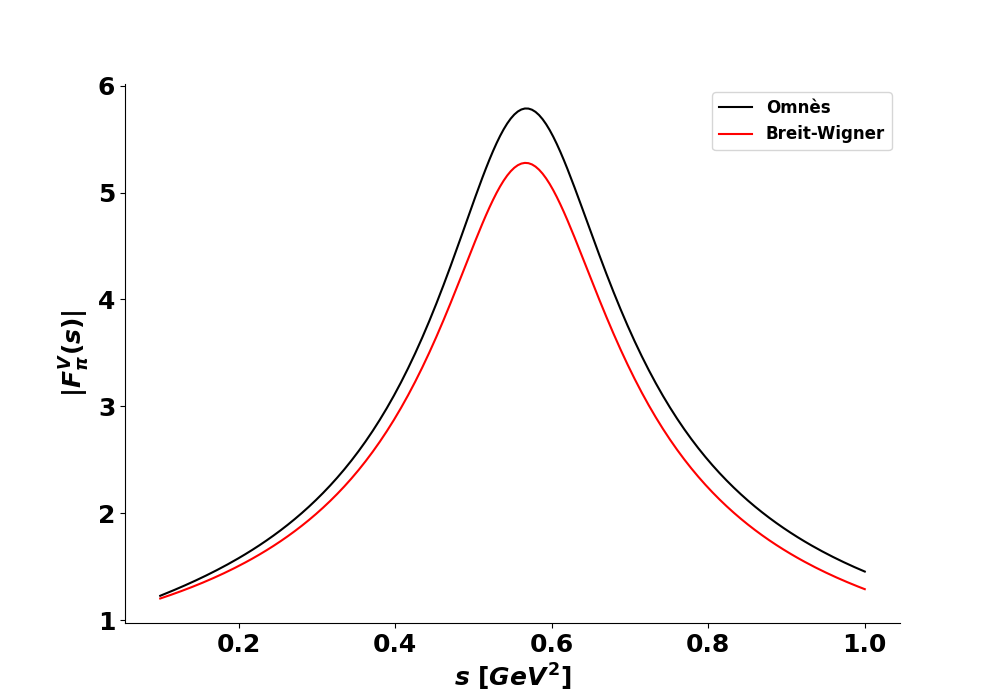
\includegraphics[width=0.9\textwidth]{./omnes_bw.png}
    \caption{Plot of the modulus of the Breit-Wigner(red) and the Omn\`es
    representation(black) of the pion Vector From Factor for $s \in [0, 1]$ in $GeV^2$}
\end{figure}
The code for the plots and some minor calculations e.g. numerical integration
can be found in \cite{code}.

\nocite{mathe}
\nocite{stoffer}
\nocite{omnes}
\printbibliography
\end{document}
